\documentclass{article}
\usepackage{graphicx}
\title{\textbf{Step by step NFA to DFA conversion}}
\author{Generated automatically}
\begin{document}
\maketitle
\begin{center}
\section{Input NFA}
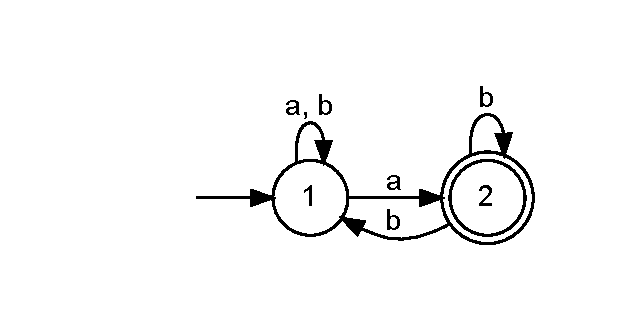
\includegraphics[width=\textwidth]{step0.dot.pdf}
\end{center}
\begin{center}
\section{Deleting lambda transitions}
\end{center}
\begin{enumerate}
\item Step 1
\begin{center}
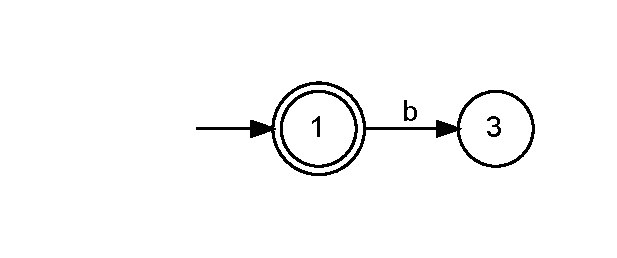
\includegraphics[width=\textwidth]{step1.dot.pdf}
\end{center}
\item Step 2
\begin{center}
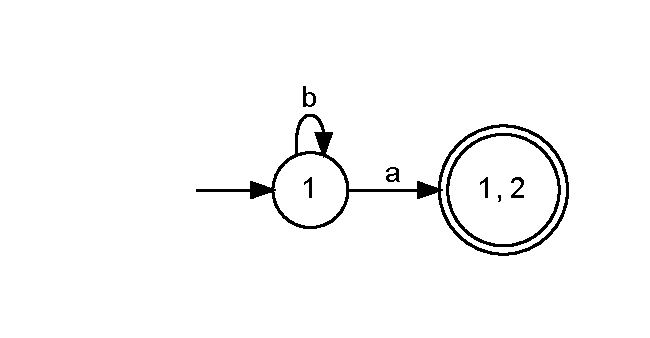
\includegraphics[width=\textwidth]{step2.dot.pdf}
\end{center}
\item Step 3
\begin{center}
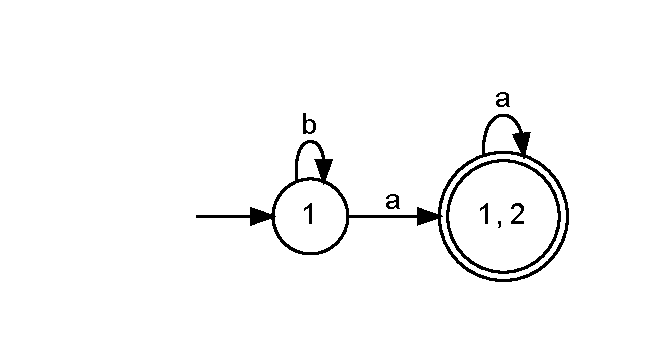
\includegraphics[width=\textwidth]{step3.dot.pdf}
\end{center}
\item Step 4
\begin{center}
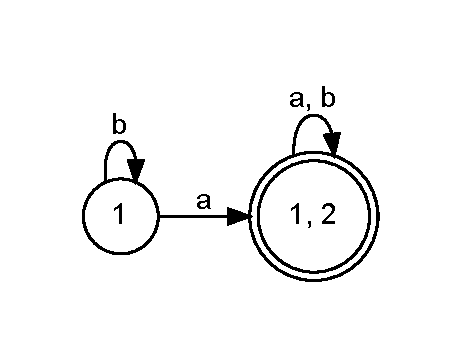
\includegraphics[width=\textwidth]{step4.dot.pdf}
\end{center}
\item Step 5
\begin{center}
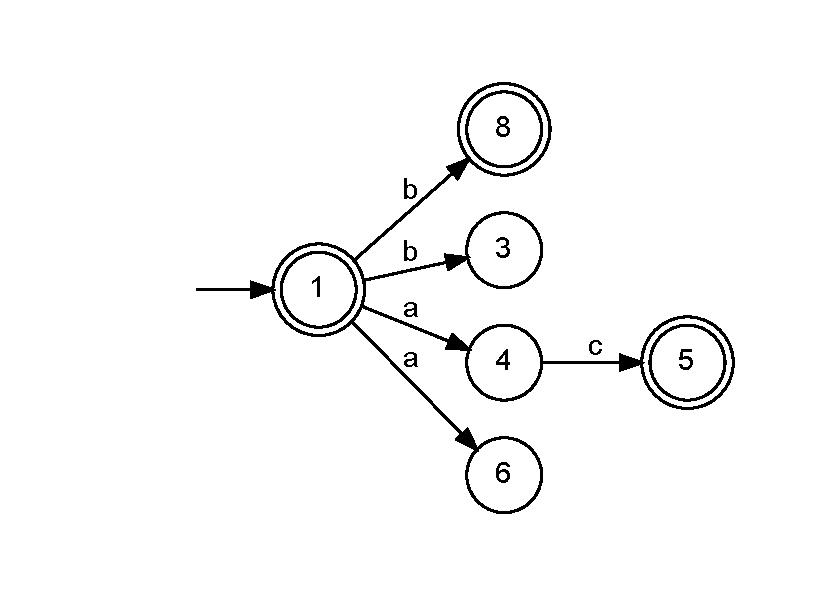
\includegraphics[width=\textwidth]{step5.dot.pdf}
\end{center}
\item Step 6
\begin{center}
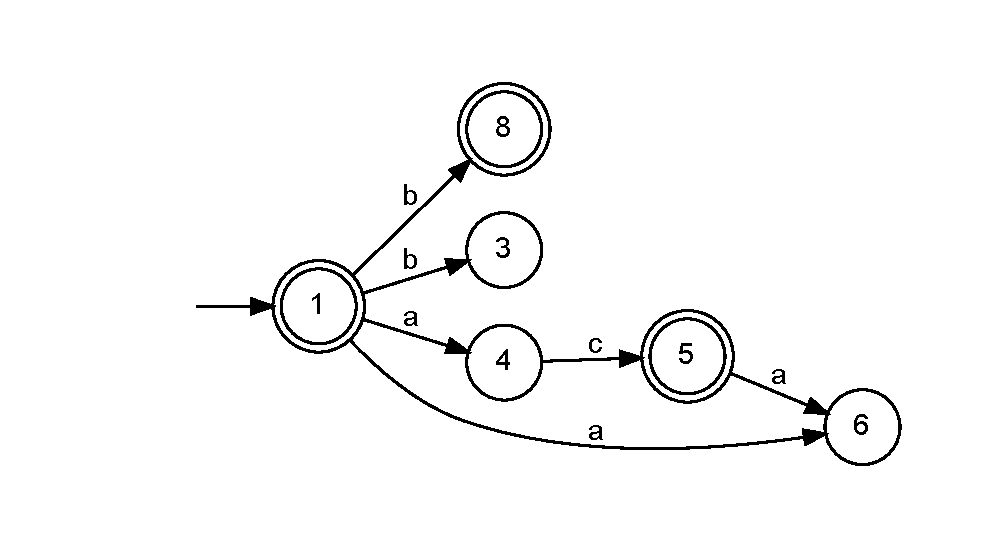
\includegraphics[width=\textwidth]{step6.dot.pdf}
\end{center}
\item Step 7
\begin{center}
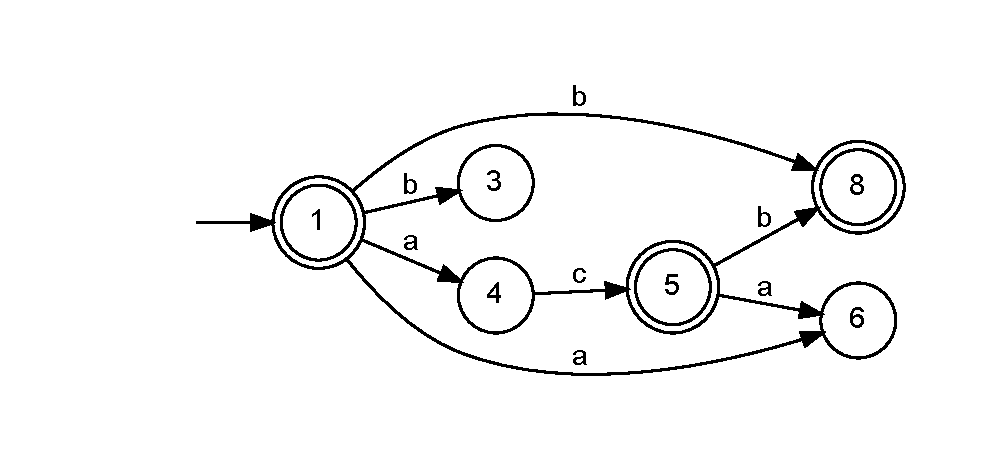
\includegraphics[width=\textwidth]{step7.dot.pdf}
\end{center}
\end{enumerate}\begin{center}
\section{Determinating}
\end{center}
\begin{enumerate}
\item Step 1
\begin{center}
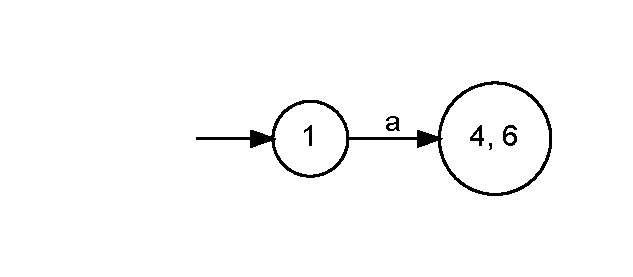
\includegraphics[width=\textwidth]{step8.dot.pdf}
\end{center}
\item Step 2
\begin{center}
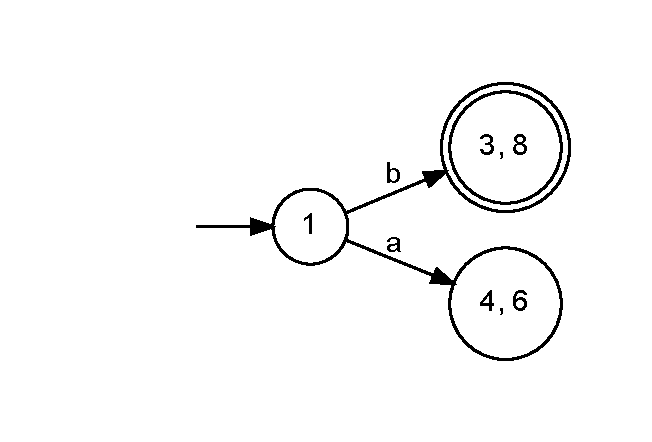
\includegraphics[width=\textwidth]{step9.dot.pdf}
\end{center}
\item Step 3
\begin{center}
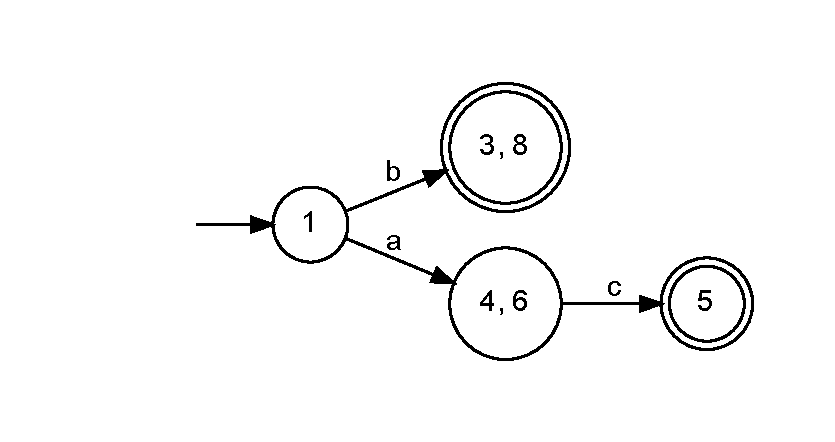
\includegraphics[width=\textwidth]{step10.dot.pdf}
\end{center}
\item Step 4
\begin{center}
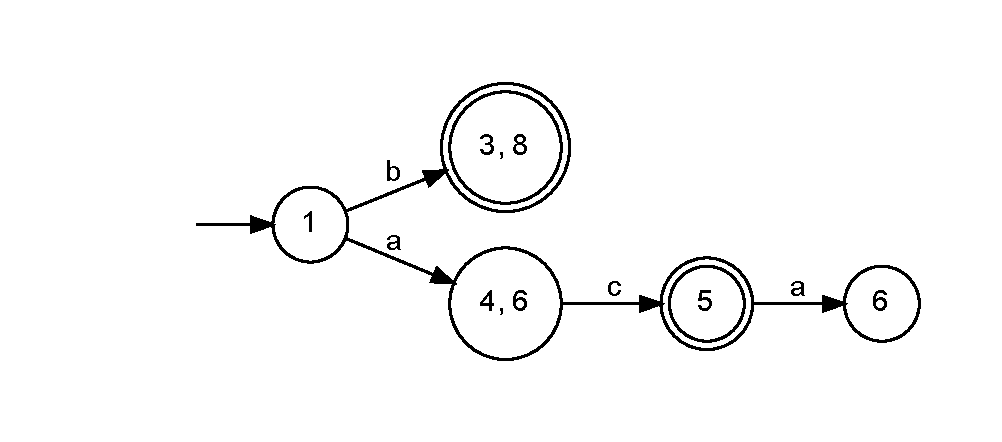
\includegraphics[width=\textwidth]{step11.dot.pdf}
\end{center}
\item Step 5
\begin{center}
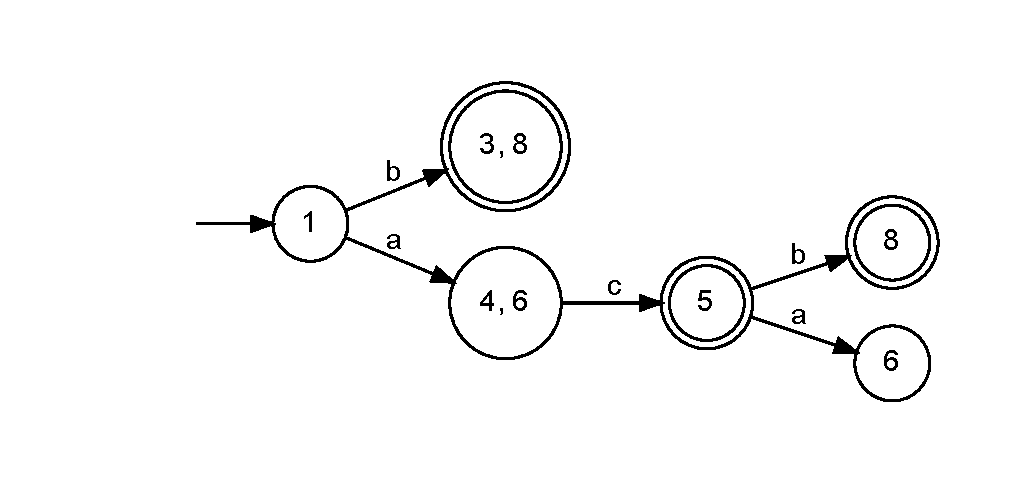
\includegraphics[width=\textwidth]{step12.dot.pdf}
\end{center}
\end{enumerate}\end{document}